\subsection{Sistema de notificações}

Um das informações disponibilizadas na página inicial de um utilizador registado é as notificações. Estas têm como objetivo informar o utilizador qual foram as atividades exercidas por outros utilizadores.

Por exemplo, para um docente, é importante que haja uma notificação, sempre que um aluno faz uma entrega num projeto. Assim evita-se que o docente esteja sempre a aceder à página de entregas para verificar se houve novas alterações.

No caso dos alunos, é importante saber que um docente lançou no sistema um novo projeto, que houve alterações no enunciado de uma fase, ou que um elemento de um dos seus grupos submeteu uma entrega.

Uma notificação está sempre associada a um projeto, portanto quando se carrega numa notificação o utilizador é redirecionado para a página do projeto respetivo.

Recorrendo-se à notificações, evita-se que um utilizador tenha que percorrer a aplicação por completo com o objetivo de verificar se ocorreram alterações no sistema.

Na página de um projeto, também são disponibilizadas notificações. Estas possuem as mesmas características das notificações existentes na página inicial.

+Na Figura~\ref{fig:notifications} pode ser consultada uma imagem demonstrativa da funcionalidade implementada.

\begin{figure}[H]
  \centering
  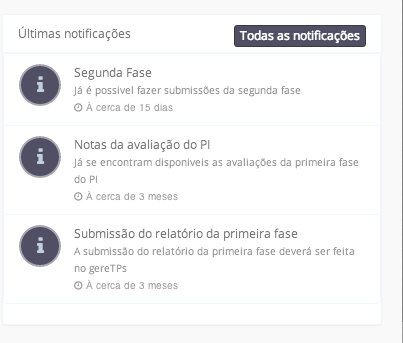
\includegraphics[width=0.65\textwidth,center]{images/implementacao/alunos/notifications}
  \caption{Notificações}
  \label{fig:notifications}
\end{figure}
